%% ma: L11-B27-0012
%% lop: 11
%% chuong: 7
%% bai: 27
%% dang: 11.27.9
%% loai: TLN
%% muc: VD
%% dap_an: "1,01"
%% nguon: "(NBV)-ĐỀ SỐ 7-MỖI NGÀY 1 ĐỀ THI 2025.pdf (D07, MỖI NGÀY 1 ĐỀ - Đề số 7), Phần III Câu 2"
%% kien_thuc: "Bài 27 (thể tích khối chóp cụt đều, thể tích khối hộp chữ nhật), góc giữa mặt bên và mặt đáy (Bài 25)"
%% trang_thai: cho-duyet
%% ly_do: "Dạng toán mới đề xuất 11.27.9 (Tỉ số thể tích khối chóp cụt tứ giác đều và khối hộp chữ nhật ghép thành ống khói (đọc từ hình chiếu)); chờ giáo viên duyệt dạng."
%% ghi_chu: "Bỏ ảnh chụp máy hút mùi (chỉ minh họa). Hình thang và hình chữ nhật dựng lại từ bản vẽ gốc (đã có các số đo x, 2x, 60 độ). Đáp án gốc 1,01 đúng (sympy: 7√3/12=1,0104)."
\begin{ex}
Một ống khói có cấu trúc gồm một khối chóp cụt tứ giác đều có thể tích $V_1$ và một khối hộp chữ nhật có thể tích $V_2$ ghép lại với nhau như hình vẽ bên dưới. Cho biết bản vẽ hình chiếu của ống khói với phương chiếu trùng với phương của một cạnh đáy khối chóp cụt, hãy tính tỉ số thể tích $\dfrac{V_1}{V_2}$, kết quả làm tròn đến hàng phần trăm.
\begin{center}
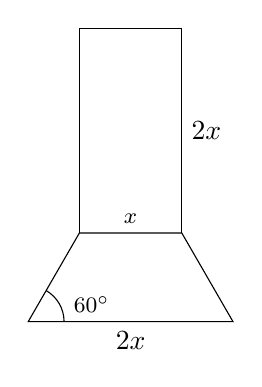
\begin{tikzpicture}[x=1.3cm,y=1.3cm]
  \def\h{0.866}
  \draw (0,0)--(2,0)--(1.5,\h)--(.5,\h)--cycle;
  \draw (.5,\h)--(.5,{\h+2})--(1.5,{\h+2})--(1.5,\h);
  \node[below] at (1,0) {$2x$};
  \node[above,font=\footnotesize] at (1,\h) {$x$};
  \node[right] at (1.5,{\h+1}) {$2x$};
  \draw (.35,0) arc[start angle=0,end angle=60,radius=.35];
  \node[font=\footnotesize] at (.62,.17) {$60^\circ$};
\end{tikzpicture}
\end{center}
\shortans{1,01}
\loigiai{Bản vẽ hình chiếu cho hình thang cân có đáy lớn $2x$, đáy nhỏ $x$, góc ở đáy $60^\circ$ (là góc giữa mặt bên và mặt đáy). Chiều cao khối chóp cụt: $h=\dfrac{2x-x}2\tan60^\circ=\dfrac{\sqrt3}2x$.

Khối chóp cụt có đáy là hình vuông cạnh $2x$ và $x$ nên
\[V_1=\dfrac h3\left(S_1+S_2+\sqrt{S_1S_2}\right)=\dfrac{\sqrt3x}{6}\left(4x^2+x^2+2x^2\right)=\dfrac{7\sqrt3}6x^3.\]

Khối hộp chữ nhật có đáy vuông cạnh $x$, cao $2x$ nên $V_2=2x^3$. Vậy $\dfrac{V_1}{V_2}=\dfrac{7\sqrt3}{12}\approx1{,}01$.}
\end{ex}
